\documentclass[12pt,article]{memoir}
% \usepackage[utf8]{inputenc}
\usepackage[T1]{fontenc}
\usepackage{tikz-uml}
\begin{document}

\newcommand{\TD}{topolog\_dim}
\newcommand{\VC}{VC}
\newcommand{\SD}{SD}
\begin{tikzpicture}
  % Draw the mesh class as a interface with two template parameters
  \umlclass[y=5,type=interface,template={real, \VC, \SD}]{mesh}{}{
    + ncells() : integer \\
    + nvertices() : integer \\
    + vertices\_of\_cell(int) : int[\VC] \\
    + coordinates\_of\_vertex(int) : real[\SD]
  }
  % Attach a note to mesh class (information about template parameters)
  \umlnote[x=7,y=6]{mesh}{real: floating point type, \\ \VC: nb. of vertices in each cell, \\ \SD: space dimension}
  % Draw the mesh1d class
  \umlclass[x=-3]{mesh1d}{}{
    + x(int): real \\
    }
  % Define mesh1d as a specialization of mesh
  \umlreal[stereo={\VC $\rightarrow$ 2, \SD $\rightarrow$ 1}]{mesh1d}{mesh}

  % Draw the mesh2d class
  \umlclass[x=3]{triang\_mesh2d}{}{
    + x(int): real \\
    + y(int): real
  }
  % Define mesh2d as a specialization of mesh
  \umlreal[stereo={\VC $\rightarrow$ 3, \SD $\rightarrow$ 2}]{triang\_mesh2d}{mesh}
\end{tikzpicture}

\end{document}                  %
